\chapter{Client}\label{Chap:Client}
The client is a web application developed in Angular. It is designed to choose and simulate the vehicle journey inside a given map.

\section{Client architecture}
The client is composed by two pages:
\begin{itemize}
	\item Home page: where it is possible to choose the path
	\item Route page: where it is possible to see the route and the next directions to take.
\end{itemize}
The application uses a service to make HTTP requests to the server to retrieve the information needed and another one to share data inside the client.
\newpage

\section{Home page}

In the home page is displayed the actual position of the vehicle in the system, if it has one, as shown in figure \ref{Fig:Position}.

\begin{figure}[!htb]
	\centering
	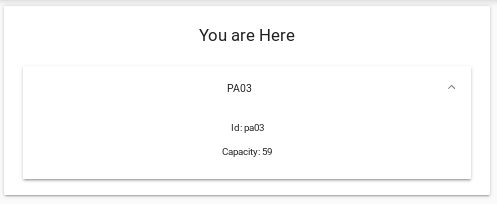
\includegraphics[width=.8\textwidth]{position.png}
	\caption{Actual position in the system.}\label{Fig:Position}
\end{figure}

All info of the places are retrieved using the API of the server \textit{/rns/webapi/rns}, starting point to obtain a map. It is then possible to decide the origin and destination of the vehicle, in order to retrieve an authorization from the server and a path that should be followed, from the list as per figure \ref{Fig:src_dst}.

\begin{figure}[!htb]
	\centering
	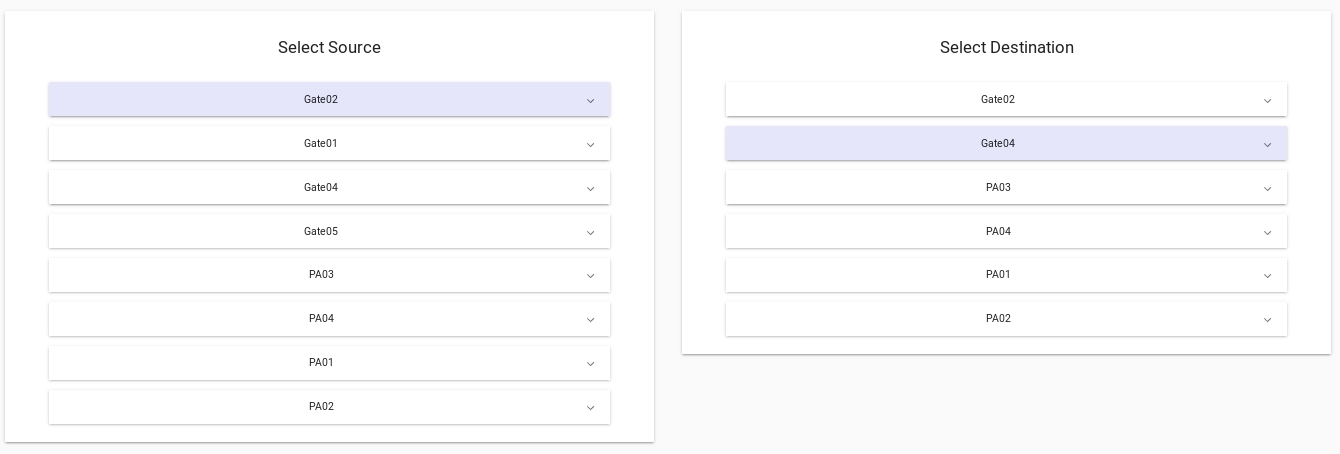
\includegraphics[width=.8\textwidth]{path_src_dst.png}
	\caption{Possible choices of source and destination.}\label{Fig:src_dst}
\end{figure}

\newpage
Also dangerous material are displayed at the end of the page, where it is possible to select only compatible materials.

\begin{figure}[!htb]
	\centering
	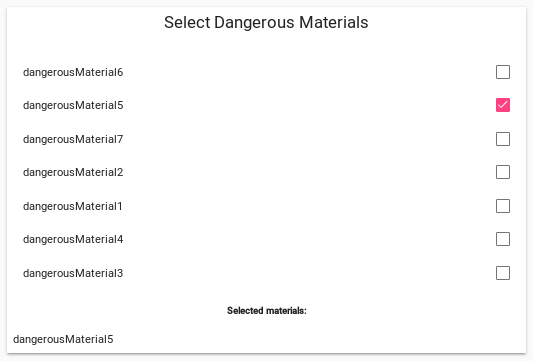
\includegraphics[width=.8\textwidth]{dangerous_mat.png}
	\caption{Possible choices of source and destination.}\label{Fig:dangerous_mat}
\end{figure}

It is then possible to create a POST request using JSON with all the information collected, that are summarized as seen in figure \ref{Fig:path_info}.

\begin{figure}[!htb]
	\centering
	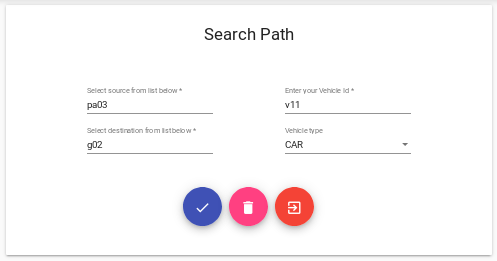
\includegraphics[width=.8\textwidth]{path_info.png}
	\caption{Possible choices of source and destination.}\label{Fig:path_info}
\end{figure}

\newpage
\section{Route page}
The client then redirects to the route page, where it is simulated the journey of the vehicle, by randomly choosing, at every crossroad, the next road to take.
It is the used a PUT request to update the position of the vehicle on the server.
The design was implemented in such way to test the correct behavior of the server in case of error.
The probability to chose a wrong road is constant and defined as 90\%. In this eventuality the server recompute a path and the client is updated.

\begin{figure}[!htb]
	\centering
	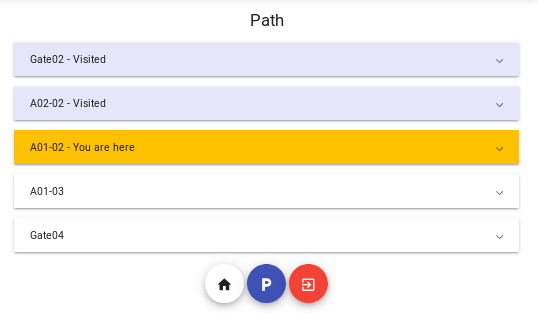
\includegraphics[width=.8\textwidth]{route_page.png}
	\caption{Simulation of the path of the vehicle.}\label{Fig:route}
\end{figure}
